\documentclass[10pt]{beamer}
\usetheme{Warsaw}
\usepackage[MeX]{polski}
\usepackage[utf8]{inputenc}
\usepackage[polish]{babel}
\usepackage{hyperref}
\usepackage{color}

\theoremstyle{definition}
\newtheorem{definicja}{Definicja}

\title[Clustering danych giełdowych]{ 
  Hurtownie Danych i Data Mining\\
  \small{Prezentacja prac nad projektem}\\
  	Wpływ wydarzeń politycznych, ekonomicznych i naturalnych
  	na kształtowanie się cen akcji na rynku polskim
 }
\author{Tomasz Kupczyk, Patryk Obara, Karol Stosiek}
\institute{Instytut Informatyki Uniwersytetu Wrocławskiego}
\date{11 maja 2010}

\begin{document}

\begin{frame}
  \titlepage
\end{frame}

\begin{frame}{Plan prezentacji}
\tableofcontents
\end{frame}

\section{Definicja problemu}

\frame{
  \begin{definicja}
  Obserwacje wahań kursów akcji pojedynczych spółek na giełdach papierów wartościowych wykazują pewną korelację z wydarzeniami politycznymi, ekonomicznymi i naturalnymi. Celem projektu jest próba zgrupowania tych spółek giełdowych w grupy wykazujące podobne zachowanie i zbadanie, które z tych grup są podatne na wydarzenia historyczne z uwzględnieniem kategorii tych wydarzeń. 
  \end{definicja}
}

\section{Plan badań}

\frame{
\begin{enumerate}
  \item Zebranie danych badawczych: notowań giełdowych wybranych spółek oraz stworzenie bazy wydarzeń historycznych.
  \item Zbudowanie wiarygodnego narzędzia do grupowania notowań spółek giełdowych oraz analizy wydarzeń historycznych
  \begin{itemize}
    \item w oparciu o algorytm k-means;
    \item z możliwością tworzenia wykresów analizowanych danych;
    \item z naniesionymi wydarzeniami historycznymi.
  \end{itemize}
  \item Dobranie odpowiednich parametrów do wiarygodnej analizy otrzymanych danych;
  \item Zanotowanie obserwacji i podjęcie próby wyciągnięcia pierwszych wniosków;
  \item Rozbudowa narzędzia o analizę opartą na sieciach Kohonena;
  \item Ponowne dobranie parametrów do analizy otrzymanych danych;
  \item Zanotowanie obserwacji i wyciągnięcie wniosków;
  \item Porównanie z wynikami osiągniętymi podczas analiz opartych o wyniki algorytmu k-means.
\end{enumerate}
}

\section{Stan prac}

\frame{
\begin{enumerate}
 \item {\bf Zebranie danych badawczych: notowań giełdowych wybranych spółek oraz stworzenie bazy wydarzeń historycznych.}
  \item {\bf Zbudowanie wiarygodnego narzędzia do grupowania notowań spółek giełdowych oraz analizy wydarzeń historycznych}
  \begin{itemize}
    \item {\bf w oparciu o algorytm k-means;}
    \item {\bf z możliwością tworzenia wykresów analizowanych danych;}
    \item {\color{gray}z naniesionymi wydarzeniami historycznymi.}
  \end{itemize}
  \item {\bf Dobranie odpowiednich parametrów do wiarygodnej analizy otrzymanych danych;}
  \item {\bf Zanotowanie obserwacji i podjęcie próby wyciągnięcia pierwszych wniosków;}
  \item {\color{gray}Rozbudowa narzędzia o analizę opartą na sieciach Kohonena;}
  \item {\color{gray}Ponowne dobranie parametrów do analizy otrzymanych danych;}
  \item {\color{gray}Zanotowanie obserwacji i wyciągnięcie wniosków;}
  \item {\color{gray}Porównanie z wynikami osiągniętymi podczas analiz opartych o wyniki algorytmu k-means.}
\end{enumerate}
}

\frame{
 \frametitle{Aktualne osiągnięcia}
 \begin{itemize}
 \item Uzupełnić.
 \end{itemize}
}

\section{Plany na przyszłość}
\frame{
\begin{enumerate}
 \item {\color{gray} Zebranie danych badawczych: notowań giełdowych wybranych spółek oraz stworzenie bazy wydarzeń historycznych.}
  \item {\color{gray} Zbudowanie wiarygodnego narzędzia do grupowania notowań spółek giełdowych oraz analizy wydarzeń historycznych}
  \begin{itemize}
    \item {\color{gray}w oparciu o algorytm k-means;}
    \item {\color{gray}z możliwością tworzenia wykresów analizowanych danych;}
    \item {\bf z naniesionymi wydarzeniami historycznymi.}
  \end{itemize}
  \item {\color{gray}Dobranie odpowiednich parametrów do wiarygodnej analizy otrzymanych danych;}
  \item {\color{gray}Zanotowanie obserwacji i podjęcie próby wyciągnięcia pierwszych wniosków;}
  \item {\bf Rozbudowa narzędzia o analizę opartą na sieciach Kohonena;}
  \item {\bf Ponowne dobranie parametrów do analizy otrzymanych danych;}
  \item {\bf Zanotowanie obserwacji i wyciągnięcie wniosków;}
  \item {\bf Porównanie z wynikami osiągniętymi podczas analiz opartych o wyniki algorytmu k-means.}
\end{enumerate}
}

\section{Używane narzędzia}

\frame{
\href{http://bonsai.ims.u-tokyo.ac.jp/~mdehoon/software/cluster/software.htm}{Pycluster}

\begin{center}

\includegraphics[scale=0.25]{python-powered.png} 
\end{center}
}

\frame{
\href{http://www.gnuplot.info/}{gnuplot}

\begin{center}
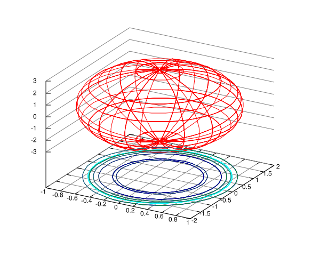
\includegraphics[scale=0.5]{gnuplot_ellipsoid.png} 
\end{center}
}

\frame{
\begin{center}
Dziękujemy za uwagę.
\end{center}
}
\end{document}